\chapter{Experimentos}

En el presente capítulo se presenta el diseño de los experimentos realizados así como los resultados obtenidos de ellos.

En esta sección se tratan los resultados obtenidos partiendo de desarrollar algunos experimentos que permiten determinar si la solución propuesta cumple con el objetivo planteado.

\section{Diseño experimental}
En la presente sección se discute el diseño de experimentos, es decir, qué valores constantes fueron utilizados para su realización y por qué se usan dichos valores.

\subsection{Datos de entrada}
Los datos de egresos hospitalarios de los años 2017 y 2018 provienen de la base de datos de la Secretaría de Salud del Gobierno de México \cite{f1}. También se tienen registros de los niveles de PM10 y PM2.5 presentes en el área metropolitana de Monterrey, dichos registros son obtenidos por las estaciones de monitoreo pertenecientes al SIMA \cite{f2} mostradas en la figura \ref{estaciones} en la página \pageref{estaciones}. Los documentos con los datos son proporcionados por \citet{f3}.

\begin{description}
\item [Selección de datos.] {Los conjuntos de datos por año de egresos hospitalarios contienen información de todos los estados de México, por lo cual se hace una limpieza de datos para solo obtener los registros de Nuevo León ya que de dicha entidad es de la cual se tienen los datos de contaminación.}
\item [Datos de ingresos hospitalarios.] {Se agrupan en semanas epidemiológicas para una mejor manipulación de ellos. Por CIE se obtiene el número de egresos en cada semana del año ordenadas por el número de egresos en el año partiendo de la CIE con la mayor cantidad.}
\item [Datos de los contaminantes.] {Se agrupan en semanas epidemiológicas para una mejor manipulación de ellos. Se obtiene el promedio del nivel del contaminante por cada semana del año.}
\end{description}

\subsection{Visualización de datos}
Con los datos ya seleccionados y agrupados se procede a generar las visualizaciones de los datos. Las visualizaciones de los datos se hacen con series de tiempo y gráficos de radar.

\begin{description}
\item [Series de tiempo.] {Se procede a generar series de tiempo de cada año por contaminante y CIE}. Las variables ajustables son:
\begin{itemize}
	\item El nombre del contaminante.
	\item El año del que se quieren obtener las series de tiempo.
	\item Número de series de tiempo a generar por contaminante. Se parte de la CIE con mayor número de egresos.
\end{itemize}

\item [Gráficos de radar.] {Los datos ya seleccionados y agrupados se normalizan teniendo como valor mínimo cero y como valor máximo un número entre uno y cuatro. Posteriormente se generan gráficos de radar de cada año por semana, en las que se muestra el nivel contaminante y la variación de las CIE}. Las variables ajustables son:
\begin{itemize}
    \item Cantidad de CIE a agregar en el gráfico. Se parte de la CIE con mayor número de egresos.
	\item Valor máximo que se utiliza para representar la longitud de los ejes en el gráfico.
	\item Nombre de la figura.
	\item Nombre de cada eje en el gráfico.
	\item Los colores de cada eje en el gráfico. 
	\item Si el gráfico es generado de forma circular o en forma de polígono.
\end{itemize}
\end{description}

\subsection{Generación de modelos}
Se procede a generar los modelos. En cada modelo se tienen métricas para evaluar su eficacia y valores que pueden ser ajustados en función de encontrar la combinación que proporcione mejores resultados.

Se tienen algunas variables que pueden ser modificadas para la generación de los modelos de regresión lineal.

\begin{itemize}
	\item Cantidad de CIE a agregar en el modelo. Se parte de la CIE con mayor número de egresos.
	\item Porcentaje de datos utilizados para el entrenamiento del modelo.
	\item Nivel de significancia.
\end{itemize}

También se tienen variables que indican información sobre la eficacia del modelo.

\begin{itemize}
	\item Valor $p$.
	\item $R^2$ (R cuadrado).
	\item Raíz de error cuadrático medio (RMSE).
\end{itemize}


\clearpage
\section{Resultados}
Establecidas las especificaciones de los experimentos que se realizan, se reportan los resultados obtenidos. Los experimentos se elaboran por contaminante, desglosando los resultados por año. En la carpeta \url{https://github.com/selenebpradop/relaciones-contaminantes-salud/tree/main/figuras/} se encuentran animaciones en video de los gráficos de radar generados por contaminante y año y todas las imágenes de las series de tiempo obtenidas.

% FORMULA PORCENTAJE ERROR
\subsection{Experimento A: Datos de niveles de PM10}
Se estudian los niveles del contaminante PM10 de los años 2017 y 2018. 

\subsubsection{Año 2017}
En la figura \ref{serie_de_tiempo_2017_PM10} se muestra una de las series de tiempo generadas para la CIE con mayor número de egresos registrados en el conjunto de datos del año. Además, en el cuadro \ref{tab:Resultados obtenidos PM10 2017} se presentan los resultados obtenidos de los modelos de regresión lineal y la eficacia obtenida de dichos modelos. El cuadro \ref{tab:RRLM PM10 2017} muestra los resultados del modelo de regresión lineal múltiple. En la figura \ref{correlaciones_2017_PM10} se muestran las correlaciones obtenidas en un gráfico de radar.

\begin{figure}[h!]
\setcounter{figure}{0} % por culpa de sciposter
\captionsetup{type=figure} % por culpa de sciposter
\begin{center}
   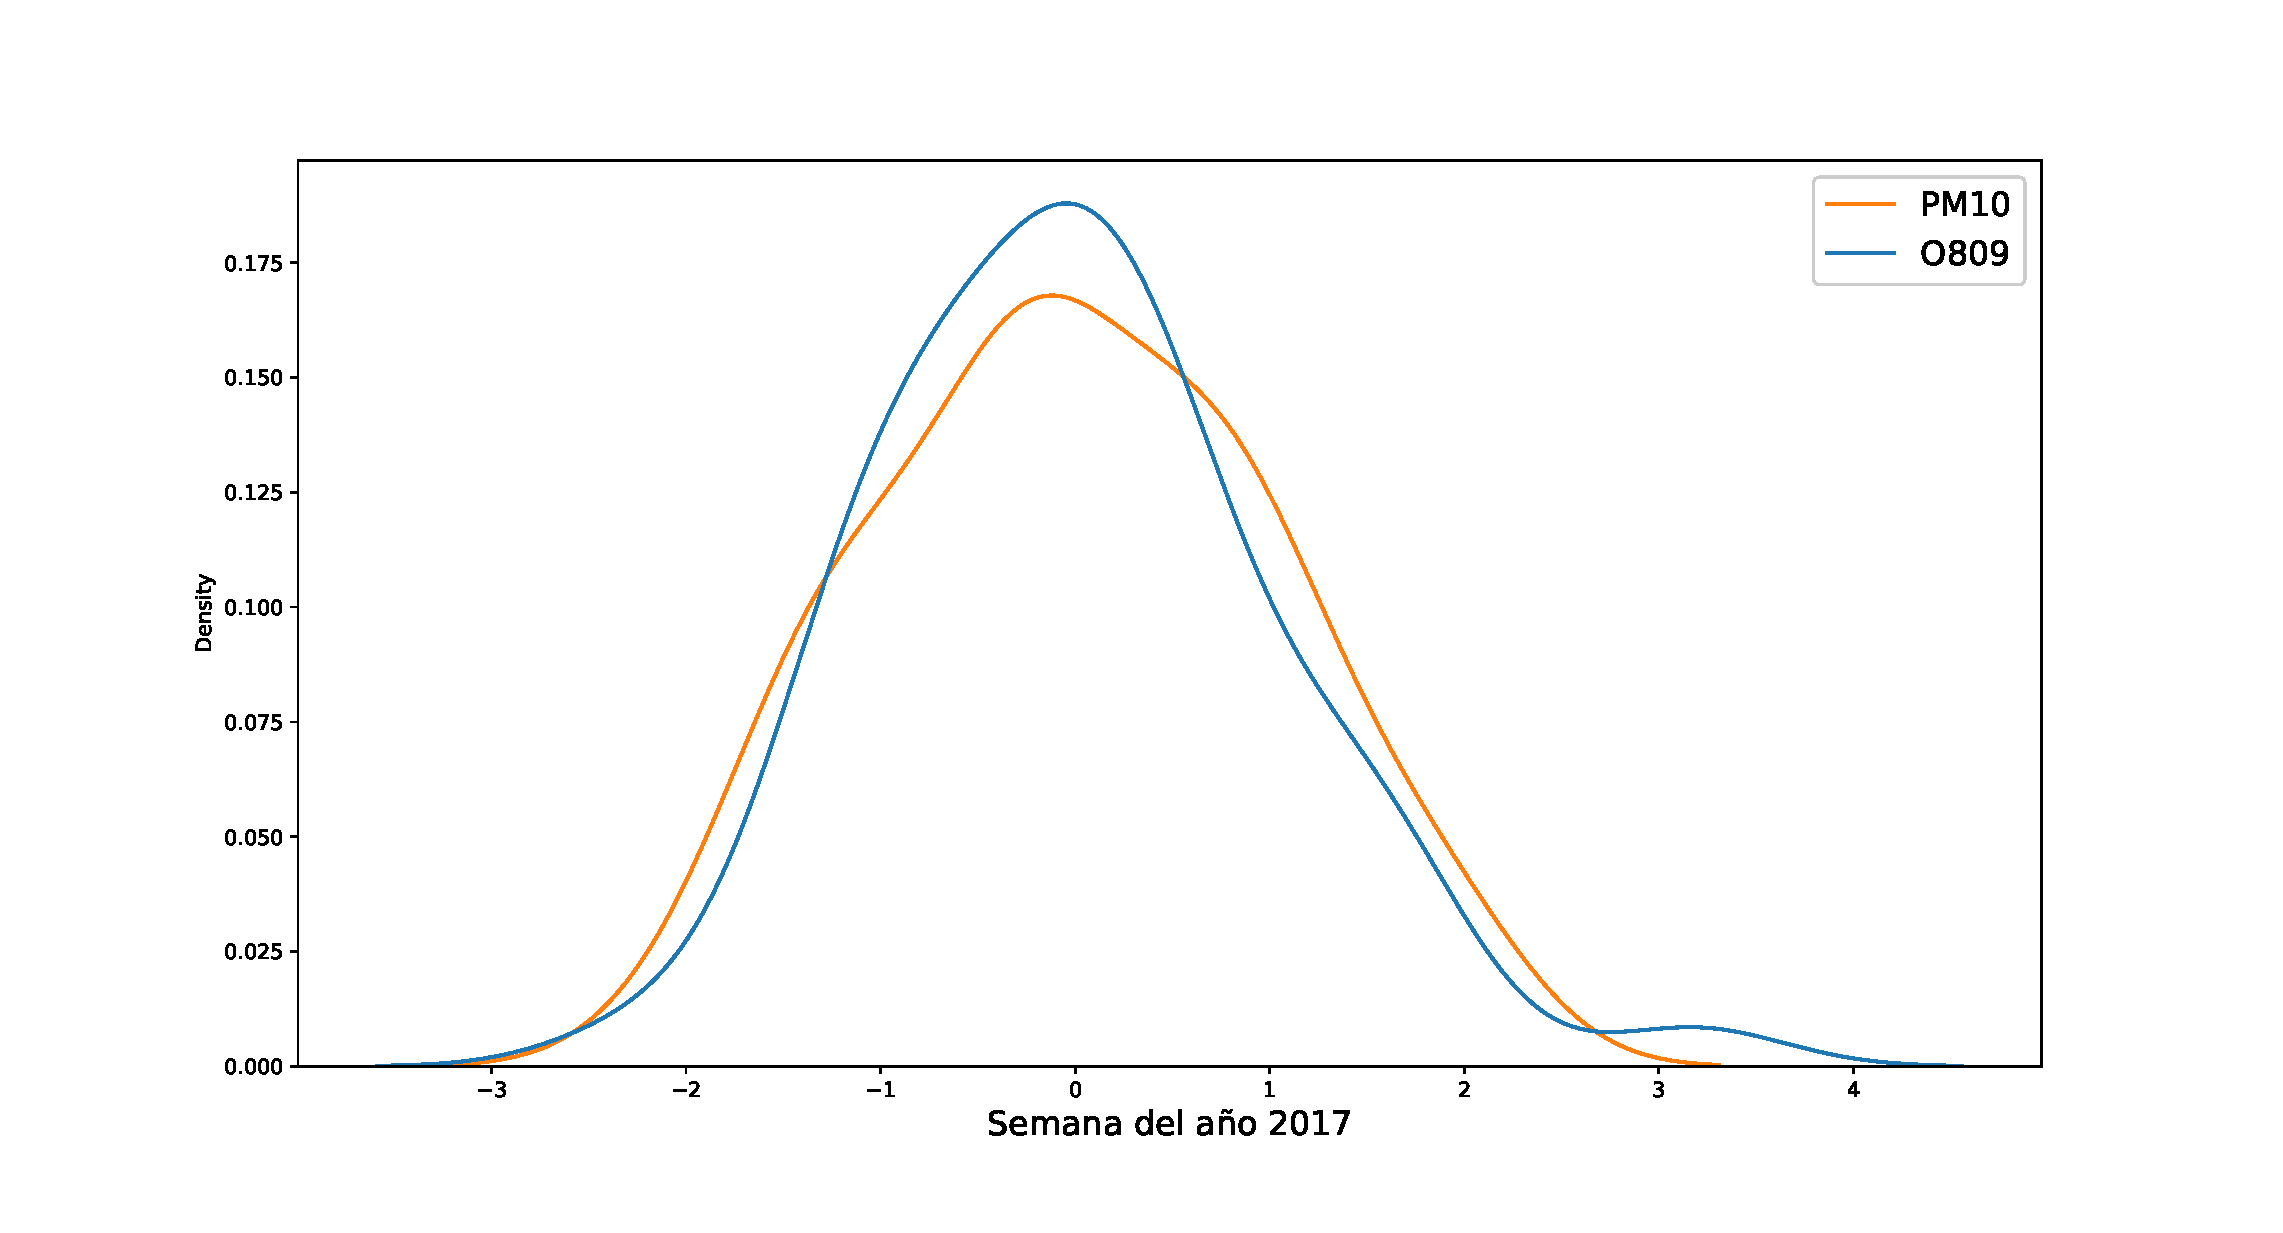
\includegraphics[trim=61 0 0 0,clip,width=1\textwidth]{PM10_O809_2017.eps}
   \end{center}
    \caption[Series de tiempo 2017 PM10 y O809]{Evolución de los niveles de PM10 y el número de egresos diagnosticados con la CIE O809 en el 2017.}
    \label{serie_de_tiempo_2017_PM10}
\end{figure}

\begin{table}[hbt!]
\centering
\caption{Resultados obtenidos PM10 2017}
\label{tab:Resultados obtenidos PM10 2017}
\vspace{0.5cm}
\begin{threeparttable}
\begin{tabular}{|c|c|c|c|c|}
	\hline
	CIE & $\rho$ & $R^2$ & Valor $p$ & $\epsilon$\\
	\hline
	O809 & -0.275 & 0.061 & 0.121 & 0.239 \\
	\hline
	O829 & 0.100 & 0.091 & 0.055 & 0.287 \\
	\hline
	O759 & -0.085 & 0.116 & 0.029 & 0.294 \\
	\hline
	O069 & -0.247 & 0.070 & 0.094 & 0.222 \\
	\hline
	K802 & 0.044 & 0.005 & 0.658 & 0.282 \\
	\hline
\end{tabular}
\begin{tablenotes}
\footnotesize
\item{$\rho$ = Coeficiente de correlación de Pearson}
\item{$\epsilon$ = RMSE para medir el error}
\end{tablenotes}
\end{threeparttable}
\end{table}

\begin{figure}[h!]
\setcounter{figure}{1} % por culpa de sciposter
\captionsetup{type=figure} % por culpa de sciposter
\begin{center}
   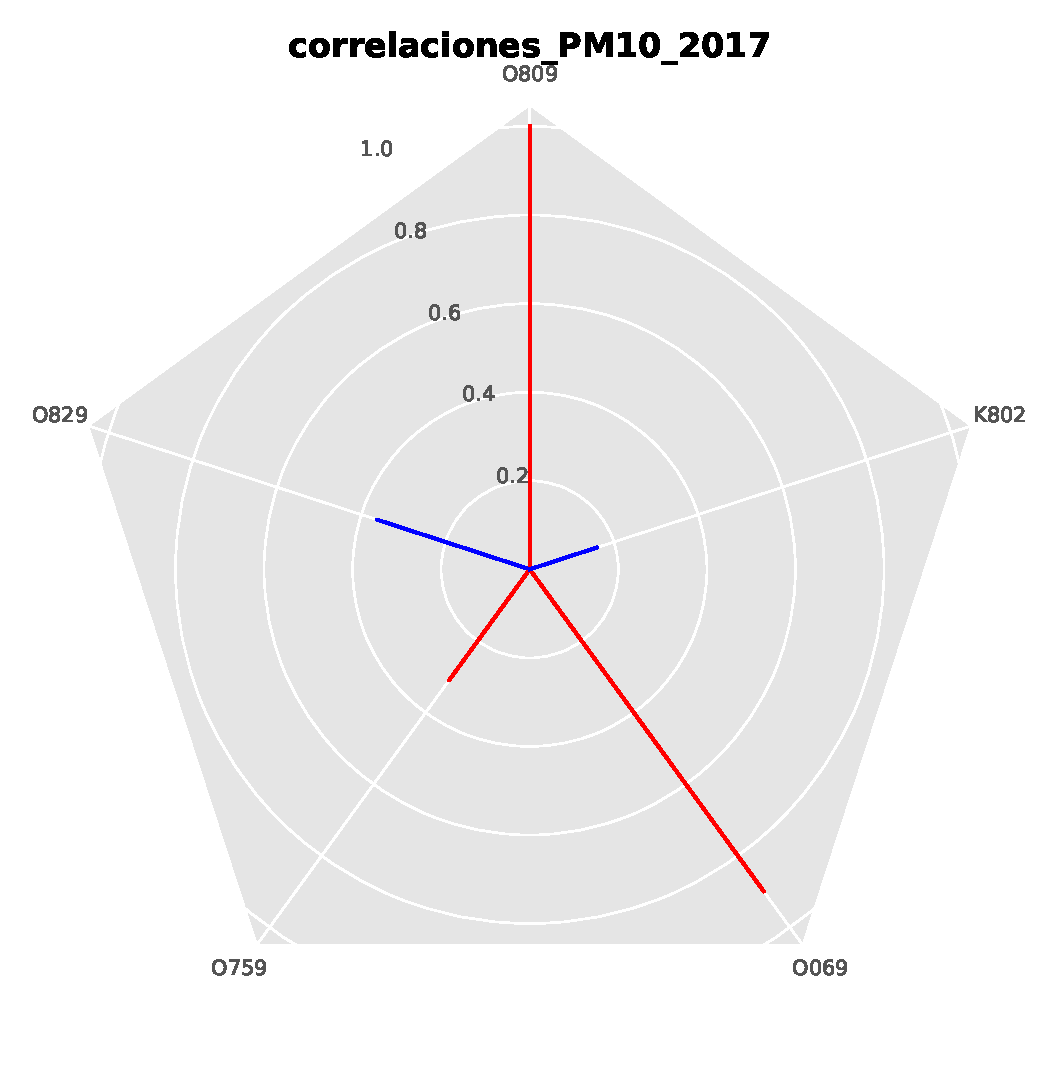
\includegraphics[trim=0 0 0 23,clip,width=1\textwidth]{spiderweb_correlaciones_PM10_2017}
   \end{center}
    \caption[Correlaciones 2017 PM10]{Correlaciones entre los niveles de PM10 y CIE en el 2017 donde el azul indica una correlación positiva y el rojo una correlación negativa.}
    \label{correlaciones_2017_PM10}
\end{figure}

\begin{table}[hbt!]
\caption{Resultados regresión lineal múltiple PM10 2017}
\label{tab:RRLM PM10 2017}
\begin{center}
\begin{tabular}{lclc}
\toprule
\textbf{Variable Dep.:}    &        $y$         & \textbf{  R$^2$:         } &     0.313   \\
\textbf{Modelo:}            &       OLS        & \textbf{Método:}           &  Mínimos cuadrados  \\
\textbf{Error:}            & 0.226  \\
\bottomrule
\end{tabular}
\begin{tabular}{lcccccc}
               & \textbf{coef} & \textbf{std err} & \textbf{$t$} & \textbf{P$> |$t$|$} & \textbf{[0.025} & \textbf{0.975]}  \\
\midrule
\textbf{const} &       0.5859  &        0.146     &     4.002  &         0.000        &        0.289    &        0.883     \\
\textbf{O809}  &      -0.3019  &        0.122     &    -2.472  &         0.018        &       -0.550    &       -0.054     \\
\textbf{O829}  &       0.2685  &        0.123     &     2.185  &         0.036        &        0.019    &        0.518     \\
\textbf{O759}  &      -0.2229  &        0.182     &    -1.222  &         0.230        &       -0.593    &        0.147     \\
\textbf{O069}  &      -0.1441  &        0.120     &    -1.200  &         0.238        &       -0.388    &        0.100     \\
\textbf{K802}  &      -0.0456  &        0.133     &    -0.344  &         0.733        &       -0.315    &        0.224     \\
\bottomrule
\end{tabular}
\end{center}
\end{table}

\clearpage
\subsubsection{Año 2018}
En la figura \ref{serie_de_tiempo_2018_PM10} se muestra una de las series de tiempo generadas para la CIE con mayor número de egresos registrados en el conjunto de datos del año. Además, en el cuadro \ref{tab:Resultados obtenidos PM10 2018} se presentan los resultados obtenidos de los modelos de regresión lineal y la eficacia obtenida de dichos modelos. El cuadro \ref{tab:RRLM PM10 2018} muestra los resultados del modelo de regresión lineal múltiple. En la figura \ref{correlaciones_2018_PM10} se muestran las correlaciones obtenidas en un gráfico de radar.

\begin{figure}[h!]
\setcounter{figure}{2} % por culpa de sciposter
\captionsetup{type=figure} % por culpa de sciposter
\begin{center}
   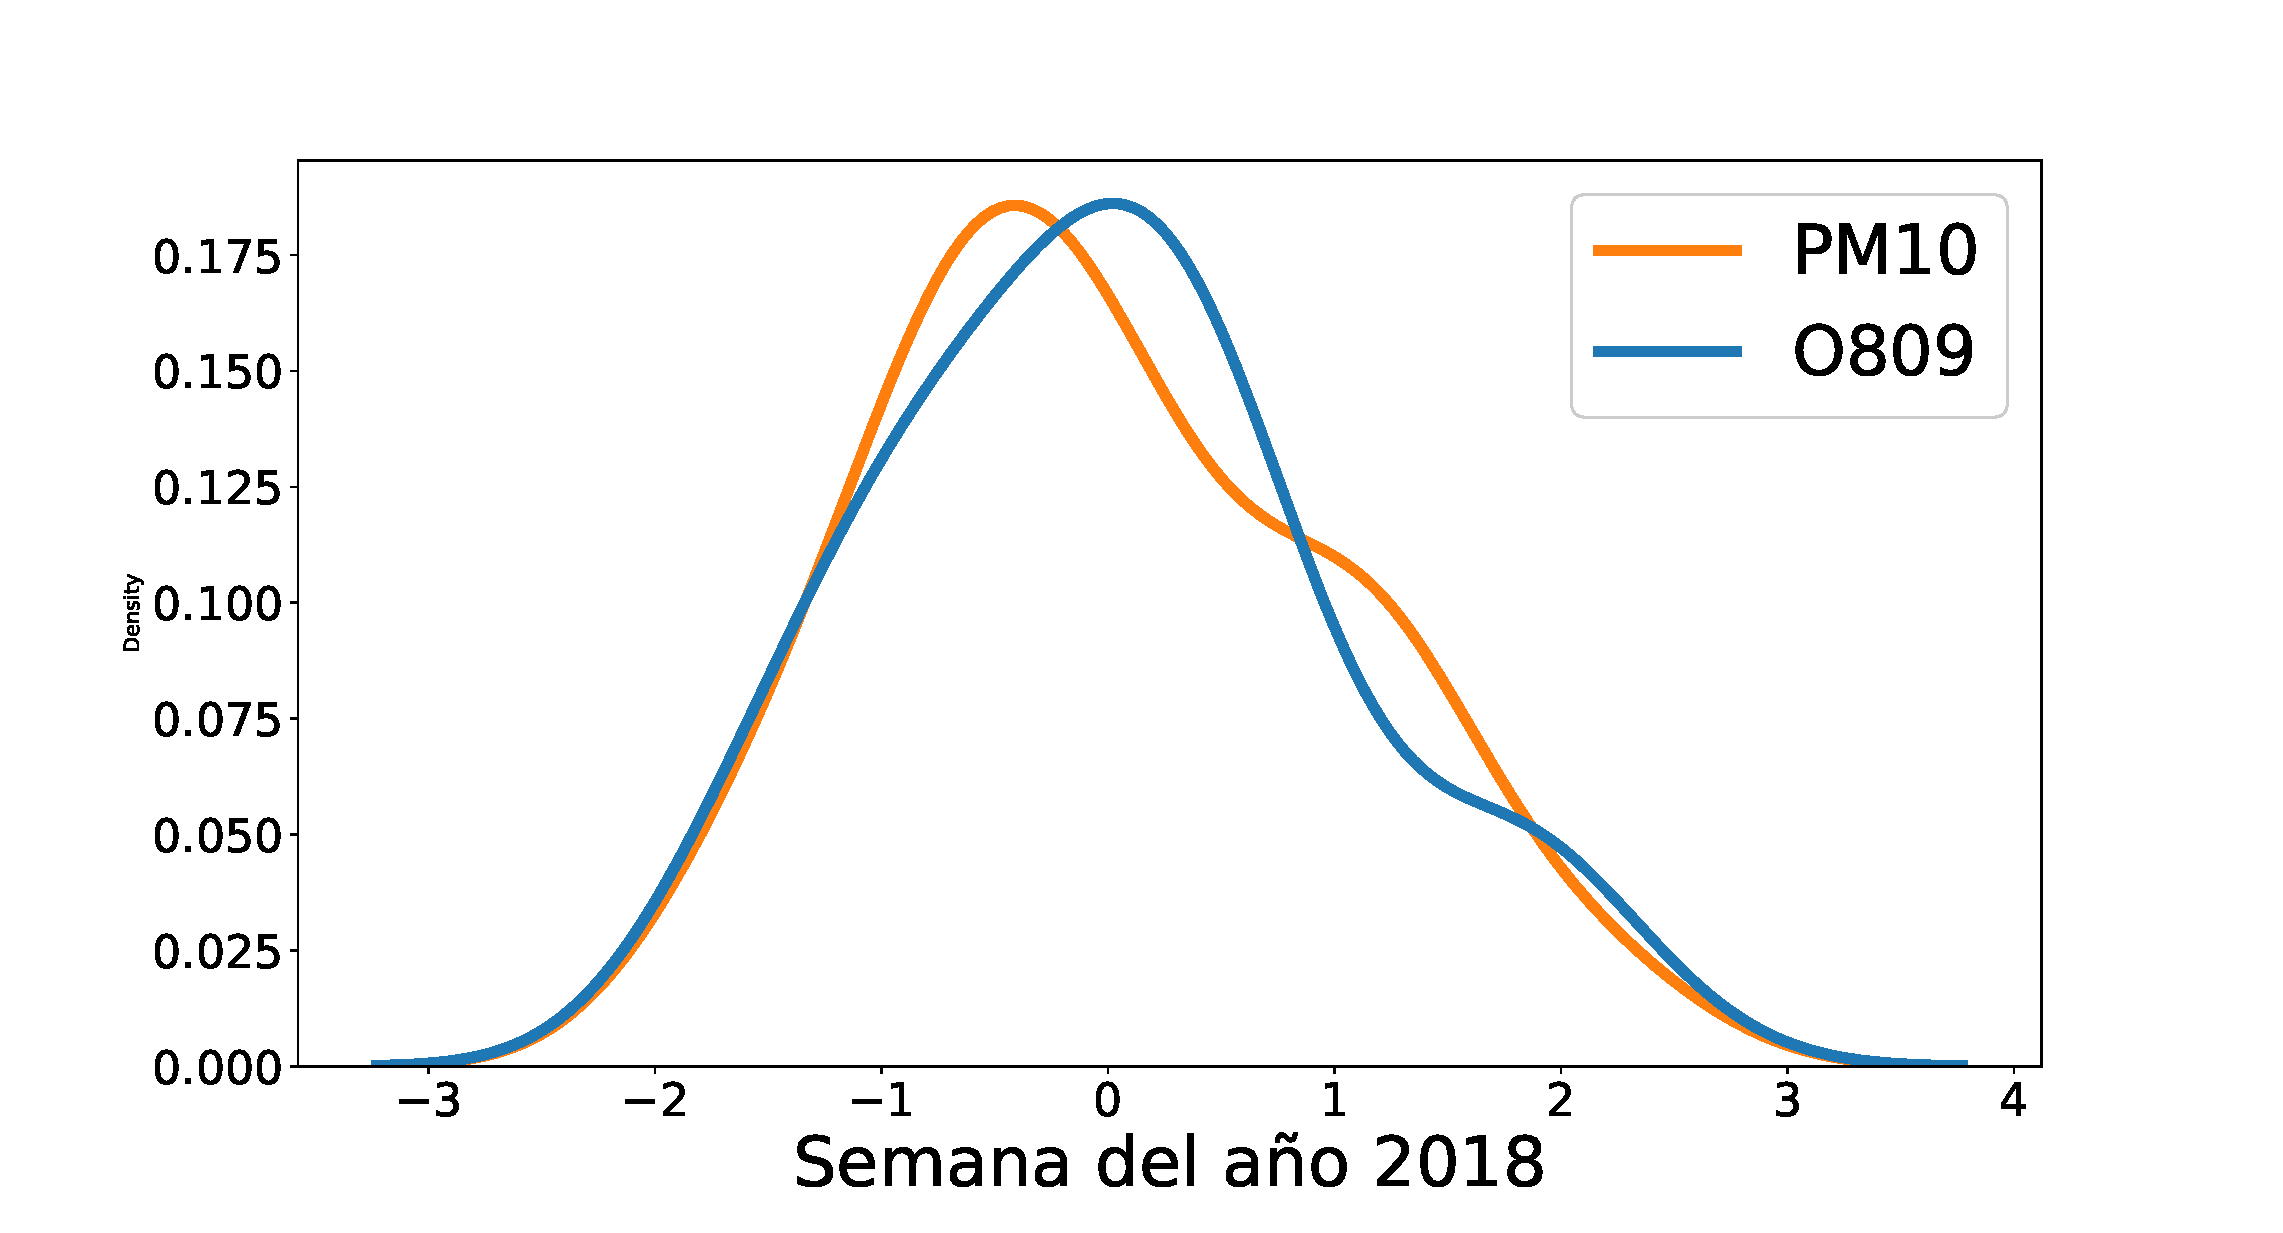
\includegraphics[trim=61 0 0 0,clip,width=1\textwidth]{PM10_O809_2018.eps}
   \end{center}
    \caption[Series de tiempo 2018 PM10 y O809]{Evolución de los niveles de PM10 y el número de egresos diagnosticados con la CIE O809 en el 2018.}
    \label{serie_de_tiempo_2018_PM10}
\end{figure}

\begin{table}[hbt!]
\centering
\caption{Resultados obtenidos PM10 2018}
\label{tab:Resultados obtenidos PM10 2018}
\vspace{0.5cm}
\begin{threeparttable}
\begin{tabular}{|c|c|c|c|c|}
	\hline
	CIE & $\rho$ & $R^2$ & Valor $p$ & $\epsilon$\\
	\hline
	O809 & -0.271 & 0.015 & 0.440 & 0.275 \\
	\hline
	O829 & 0.282 & 0.069 & 0.098 & 0.249 \\
	\hline
	K802 & 0.277 & 0.084 & 0.066 & 0.152 \\
	\hline
	O342 & -0.401 & 0.100 & 0.044 & 0.248 \\
	\hline
	N40X & -0.009 & 0.000 & 0.964 & 0.243 \\
	\hline
\end{tabular}
\begin{tablenotes}
\footnotesize
\item{$\rho$ = Coeficiente de correlación de Pearson}
\item{$\epsilon$ = RMSE para medir el error}
\end{tablenotes}
\end{threeparttable}
\end{table}

\begin{figure}[h!]
\setcounter{figure}{3} % por culpa de sciposter
\captionsetup{type=figure} % por culpa de sciposter
\begin{center}
   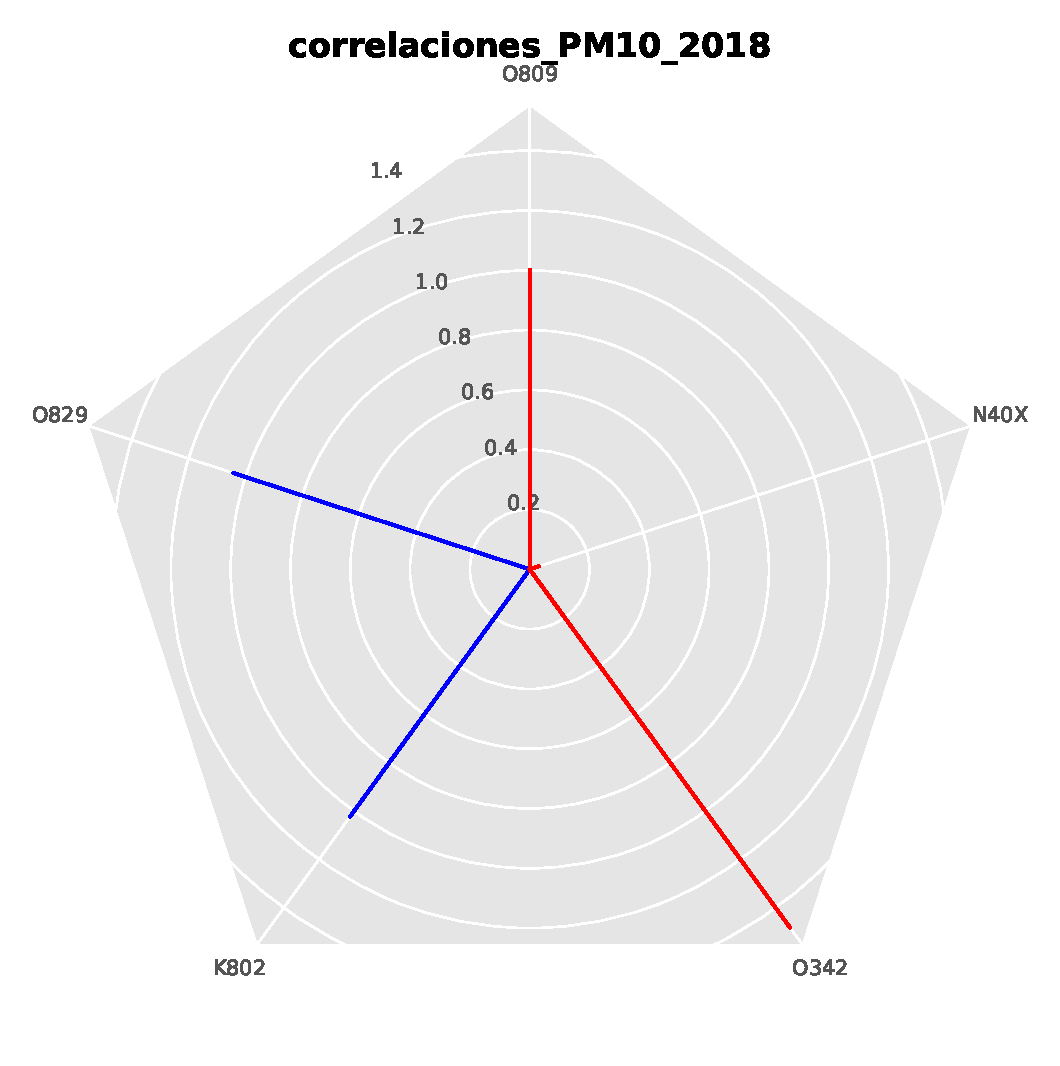
\includegraphics[trim=0 0 0 23,clip,width=1\textwidth]{spiderweb_correlaciones_PM10_2018}
   \end{center}
    \caption[Correlaciones 2018 PM10]{Correlaciones entre los niveles de PM10 y CIE en el 2018 donde el azul indica una correlación positiva y el rojo una correlación negativa.}
    \label{correlaciones_2018_PM10}
\end{figure}

\begin{table}[hbt!]
\caption{Resultados regresión lineal múltiple PM10 2018}
\label{tab:RRLM PM10 2018}
\begin{center}
\begin{tabular}{lclc}
\toprule
\textbf{Variable Dep.:}    &        $y$         & \textbf{  R$^2$:         } &     0.182   \\
\textbf{Modelo:}            &       OLS        & \textbf{Método:}           &  Mínimos cuadrados  \\
\textbf{Error:}            & 0.159  \\
\bottomrule
\end{tabular}
\begin{tabular}{lcccccc}
               & \textbf{coef} & \textbf{std err} & \textbf{$t$} & \textbf{P$> |$t$|$} & \textbf{[0.025} & \textbf{0.975]}  \\
\midrule
\textbf{const} &       0.3885  &        0.210     &     1.849  &         0.073        &       -0.038    &        0.815     \\
\textbf{O809}  &      -0.0114  &        0.188     &    -0.061  &         0.952        &       -0.392    &        0.370     \\
\textbf{O829}  &       0.0854  &        0.214     &     0.400  &         0.692        &       -0.349    &        0.520     \\
\textbf{K802}  &       0.3088  &        0.167     &     1.852  &         0.072        &       -0.030    &        0.647     \\
\textbf{O342}  &      -0.1708  &        0.208     &    -0.820  &         0.418        &       -0.593    &        0.252     \\
\textbf{N40X}  &      -0.1239  &        0.167     &    -0.740  &         0.464        &       -0.464    &        0.216     \\
\bottomrule
\end{tabular}
\end{center}
\end{table}


\clearpage
\subsection{Experimento B: Niveles de PM2.5}
Se estudian los niveles del contaminante PM2.5 de los años 2017 y 2018.

\subsubsection{Año 2017}
En la figura \ref{serie_de_tiempo_2017_PM25} se muestra una de las series de tiempo generadas para la CIE con mayor número de egresos registrados en el conjunto de datos del año. Además, en el cuadro \ref{tab:Resultados obtenidos PM2.5 2017} se presentan los resultados obtenidos de los modelos de regresión lineal y la eficacia obtenida de dichos modelos. El cuadro \ref{tab:RRLM PM2.5 2017} muestra los resultados del modelo de regresión lineal múltiple. En la figura \ref{correlaciones_2017_PM25} se muestran las correlaciones obtenidas en un gráfico de radar.

\begin{figure}[h!]
\setcounter{figure}{4} % por culpa de sciposter
\captionsetup{type=figure} % por culpa de sciposter
\begin{center}
   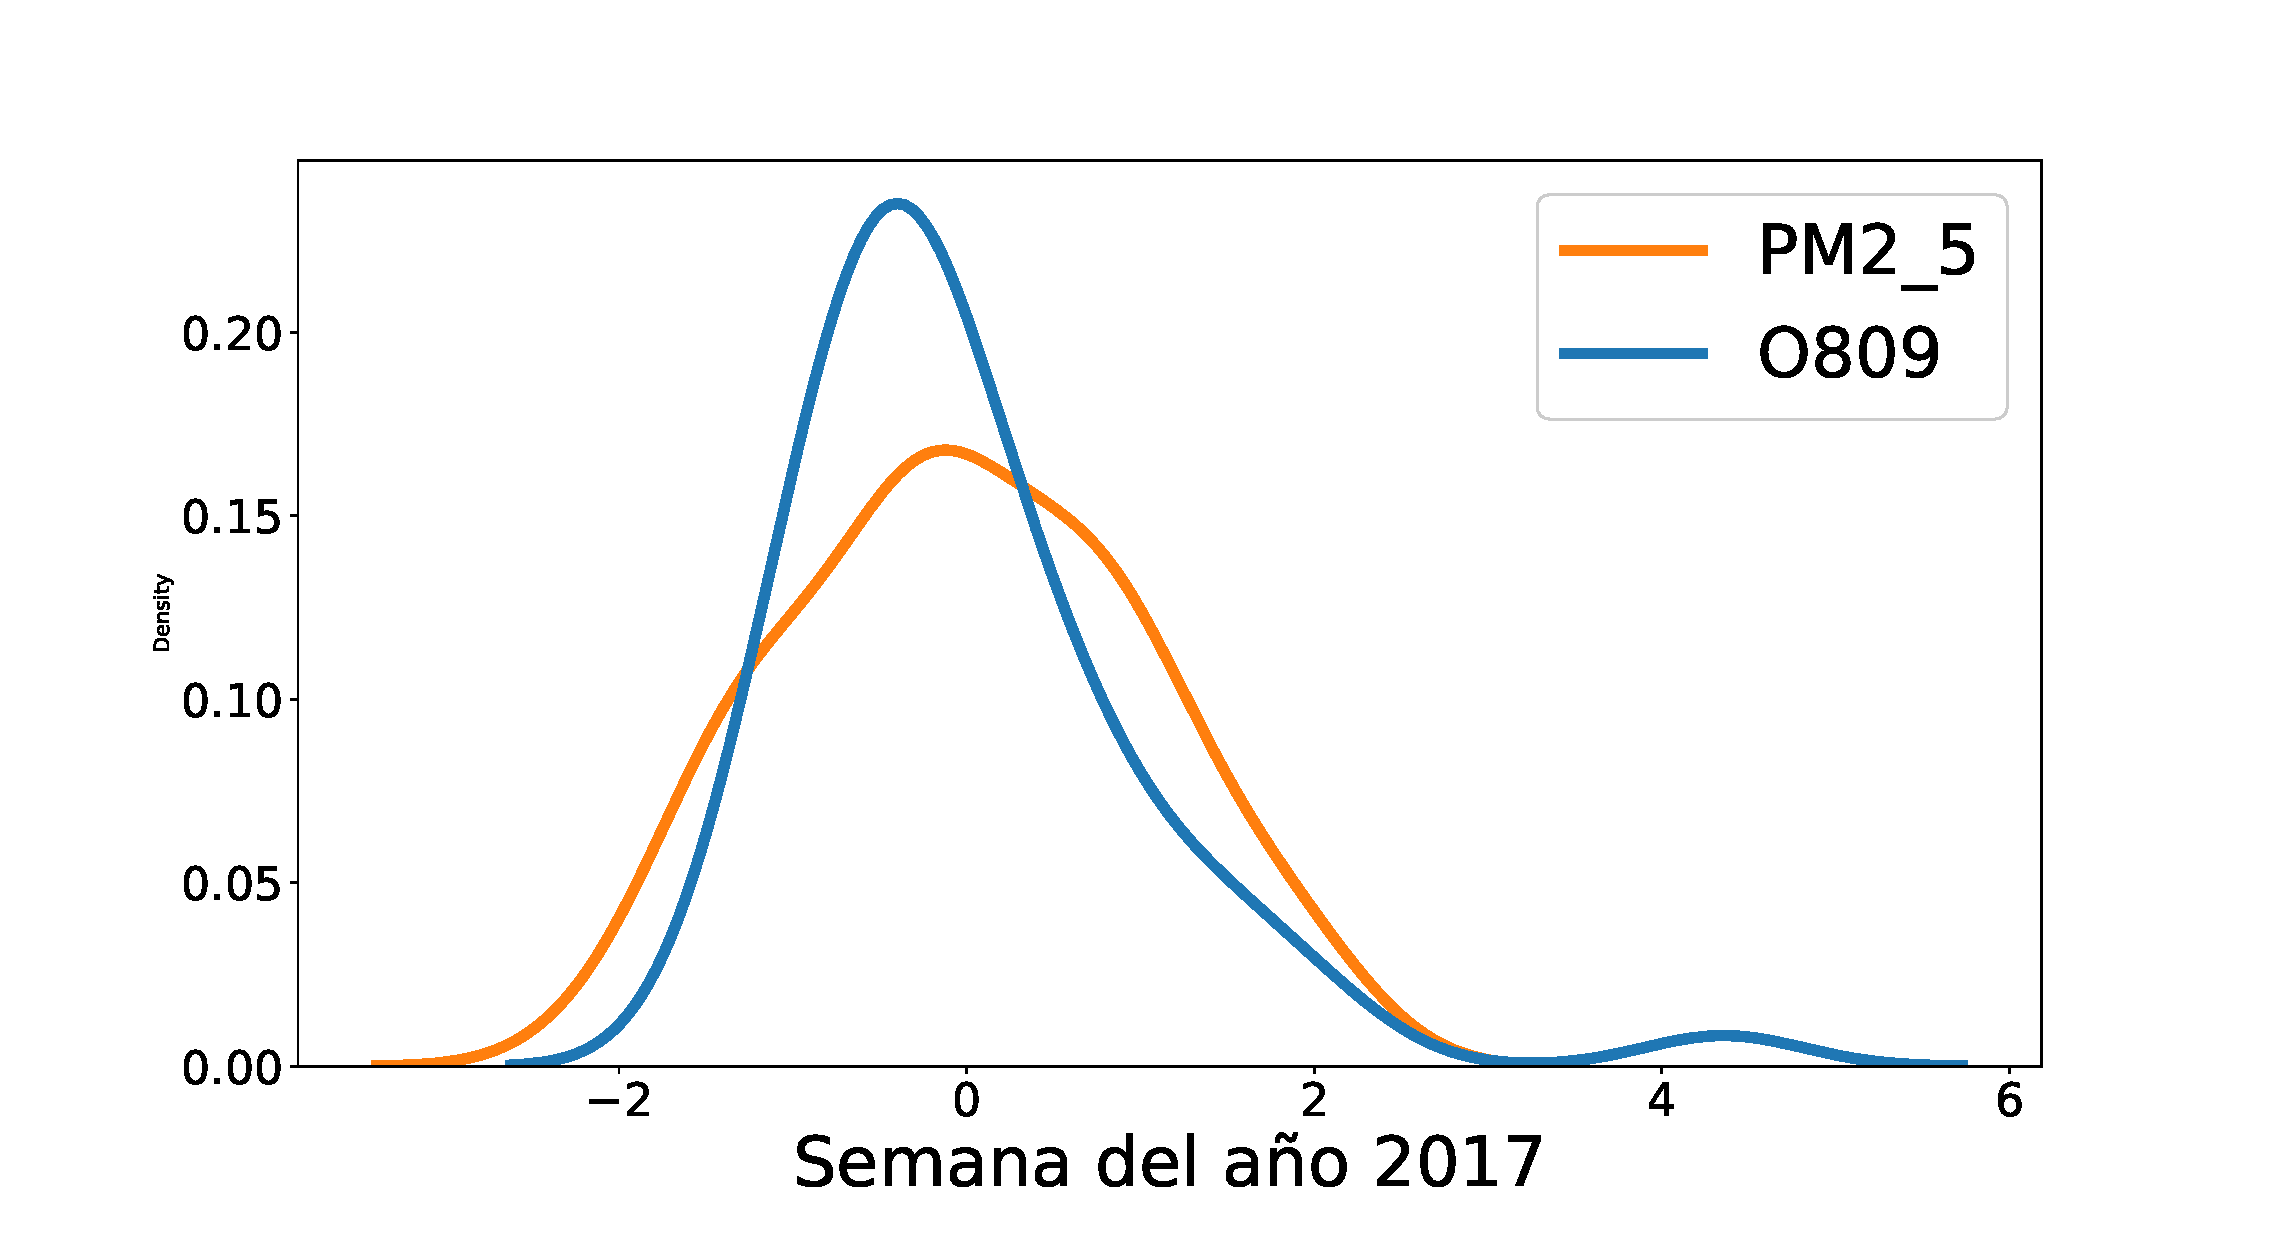
\includegraphics[trim=61 0 0 0,clip,width=1\textwidth]{PM2_5_O809_2017.eps}
   \end{center}
    \caption[Series de tiempo 2017 PM2.5 y O809]{Evolución de los niveles de PM2.5 y el número de egresos diagnosticados con la CIE O809 en el 2017.}
    \label{serie_de_tiempo_2017_PM25}
\end{figure}

\begin{table}[hbt!]
\centering
\caption{Resultados obtenidos PM2.5 2017}
\label{tab:Resultados obtenidos PM2.5 2017}
\vspace{0.5cm}
\begin{threeparttable}
\begin{tabular}{|c|c|c|c|c|}
	\hline
	CIE & $\rho$ & $R^2$ & Valor $p$ & $\epsilon$\\
	\hline
	O809 & -0.093 & 0.011 & 0.511 & 0.256 \\
	\hline
	O829 & 0.014 & 0.021 & 0.371 & 0.253 \\
	\hline
	O759 & -0.172 & 0.113 & 0.032 & 0.278 \\
	\hline
	O069 & -0.350 & 0.112 & 0.033 & 0.208 \\
	\hline
	K802 & 0.006 & 0.005 & 0.667 & 0.285 \\
	\hline
\end{tabular}
\begin{tablenotes}
\footnotesize
\item{$\rho$ = Coeficiente de correlación de Pearson}
\item{$\epsilon$ = RMSE para medir el error}
\end{tablenotes}
\end{threeparttable}
\end{table}

\begin{figure}[h!]
\setcounter{figure}{5} % por culpa de sciposter
\captionsetup{type=figure} % por culpa de sciposter
\begin{center}
   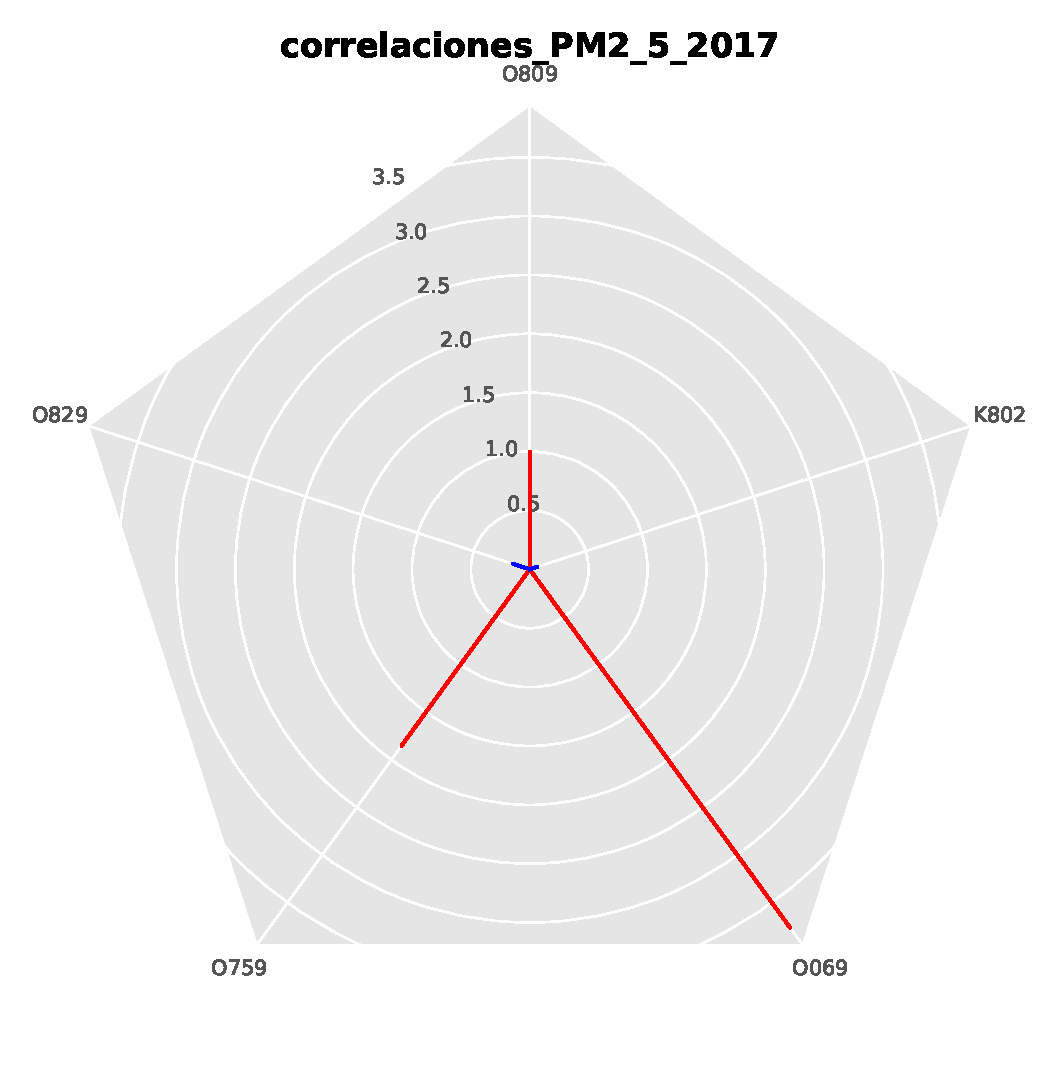
\includegraphics[trim=0 0 0 23,clip,width=1\textwidth]{spiderweb_correlaciones_PM2_5_2017}
   \end{center}
    \caption[Correlaciones 2017 PM2.5]{Correlaciones entre los niveles de PM2.5 y CIE en el 2017 donde el azul indica una correlación positiva y el rojo una correlación negativa.}
    \label{correlaciones_2017_PM25}
\end{figure}

\begin{table}[hbt!]
\caption{Resultados regresión lineal múltiple PM2.5 2017}
\label{tab:RRLM PM2.5 2017}
\begin{center}
\begin{tabular}{lclc}
\toprule
\textbf{Variable Dep.:}    &        $y$         & \textbf{  R$^2$:         } &     0.210   \\
\textbf{Modelo:}            &       OLS        & \textbf{Método:}           &  Mínimos cuadrados   \\
\textbf{Error:}            & 0.175  \\
\bottomrule
\end{tabular}
\begin{tabular}{lcccccc}
               & \textbf{coef} & \textbf{std err} & \textbf{$t$} & \textbf{P$> |$t$|$} & \textbf{[0.025} & \textbf{0.975]}  \\
\midrule
\textbf{const} &       0.5345  &        0.158     &     3.373  &         0.002        &        0.213    &        0.856     \\
\textbf{O809}  &      -0.1754  &        0.132     &    -1.327  &         0.193        &       -0.444    &        0.093     \\
\textbf{O829}  &       0.0701  &        0.133     &     0.527  &         0.602        &       -0.200    &        0.340     \\
\textbf{O759}  &      -0.2585  &        0.197     &    -1.309  &         0.199        &       -0.659    &        0.142     \\
\textbf{O069}  &      -0.2148  &        0.130     &    -1.652  &         0.108        &       -0.479    &        0.049     \\
\textbf{K802}  &      -0.1164  &        0.144     &    -0.811  &         0.423        &       -0.408    &        0.175     \\
\bottomrule
\end{tabular}
\end{center}
\end{table}

\clearpage
\subsubsection{Año 2018}
En la figura \ref{serie_de_tiempo_2018_PM25} se muestra una de las series de tiempo generadas para la CIE con mayor número de egresos registrados en el conjunto de datos del año. Además, en el cuadro \ref{tab:Resultados obtenidos PM2.5 2018} se presentan los resultados obtenidos de los modelos de regresión lineal y la eficacia obtenida de dichos modelos. El cuadro \ref{tab:RRLM PM2.5 2018} muestra los resultados del modelo de regresión lineal múltiple. En la figura \ref{correlaciones_2018_PM25} se muestran las correlaciones obtenidas en un gráfico de radar.

\begin{figure}[h!]
\setcounter{figure}{6} % por culpa de sciposter
\captionsetup{type=figure} % por culpa de sciposter
\begin{center}
   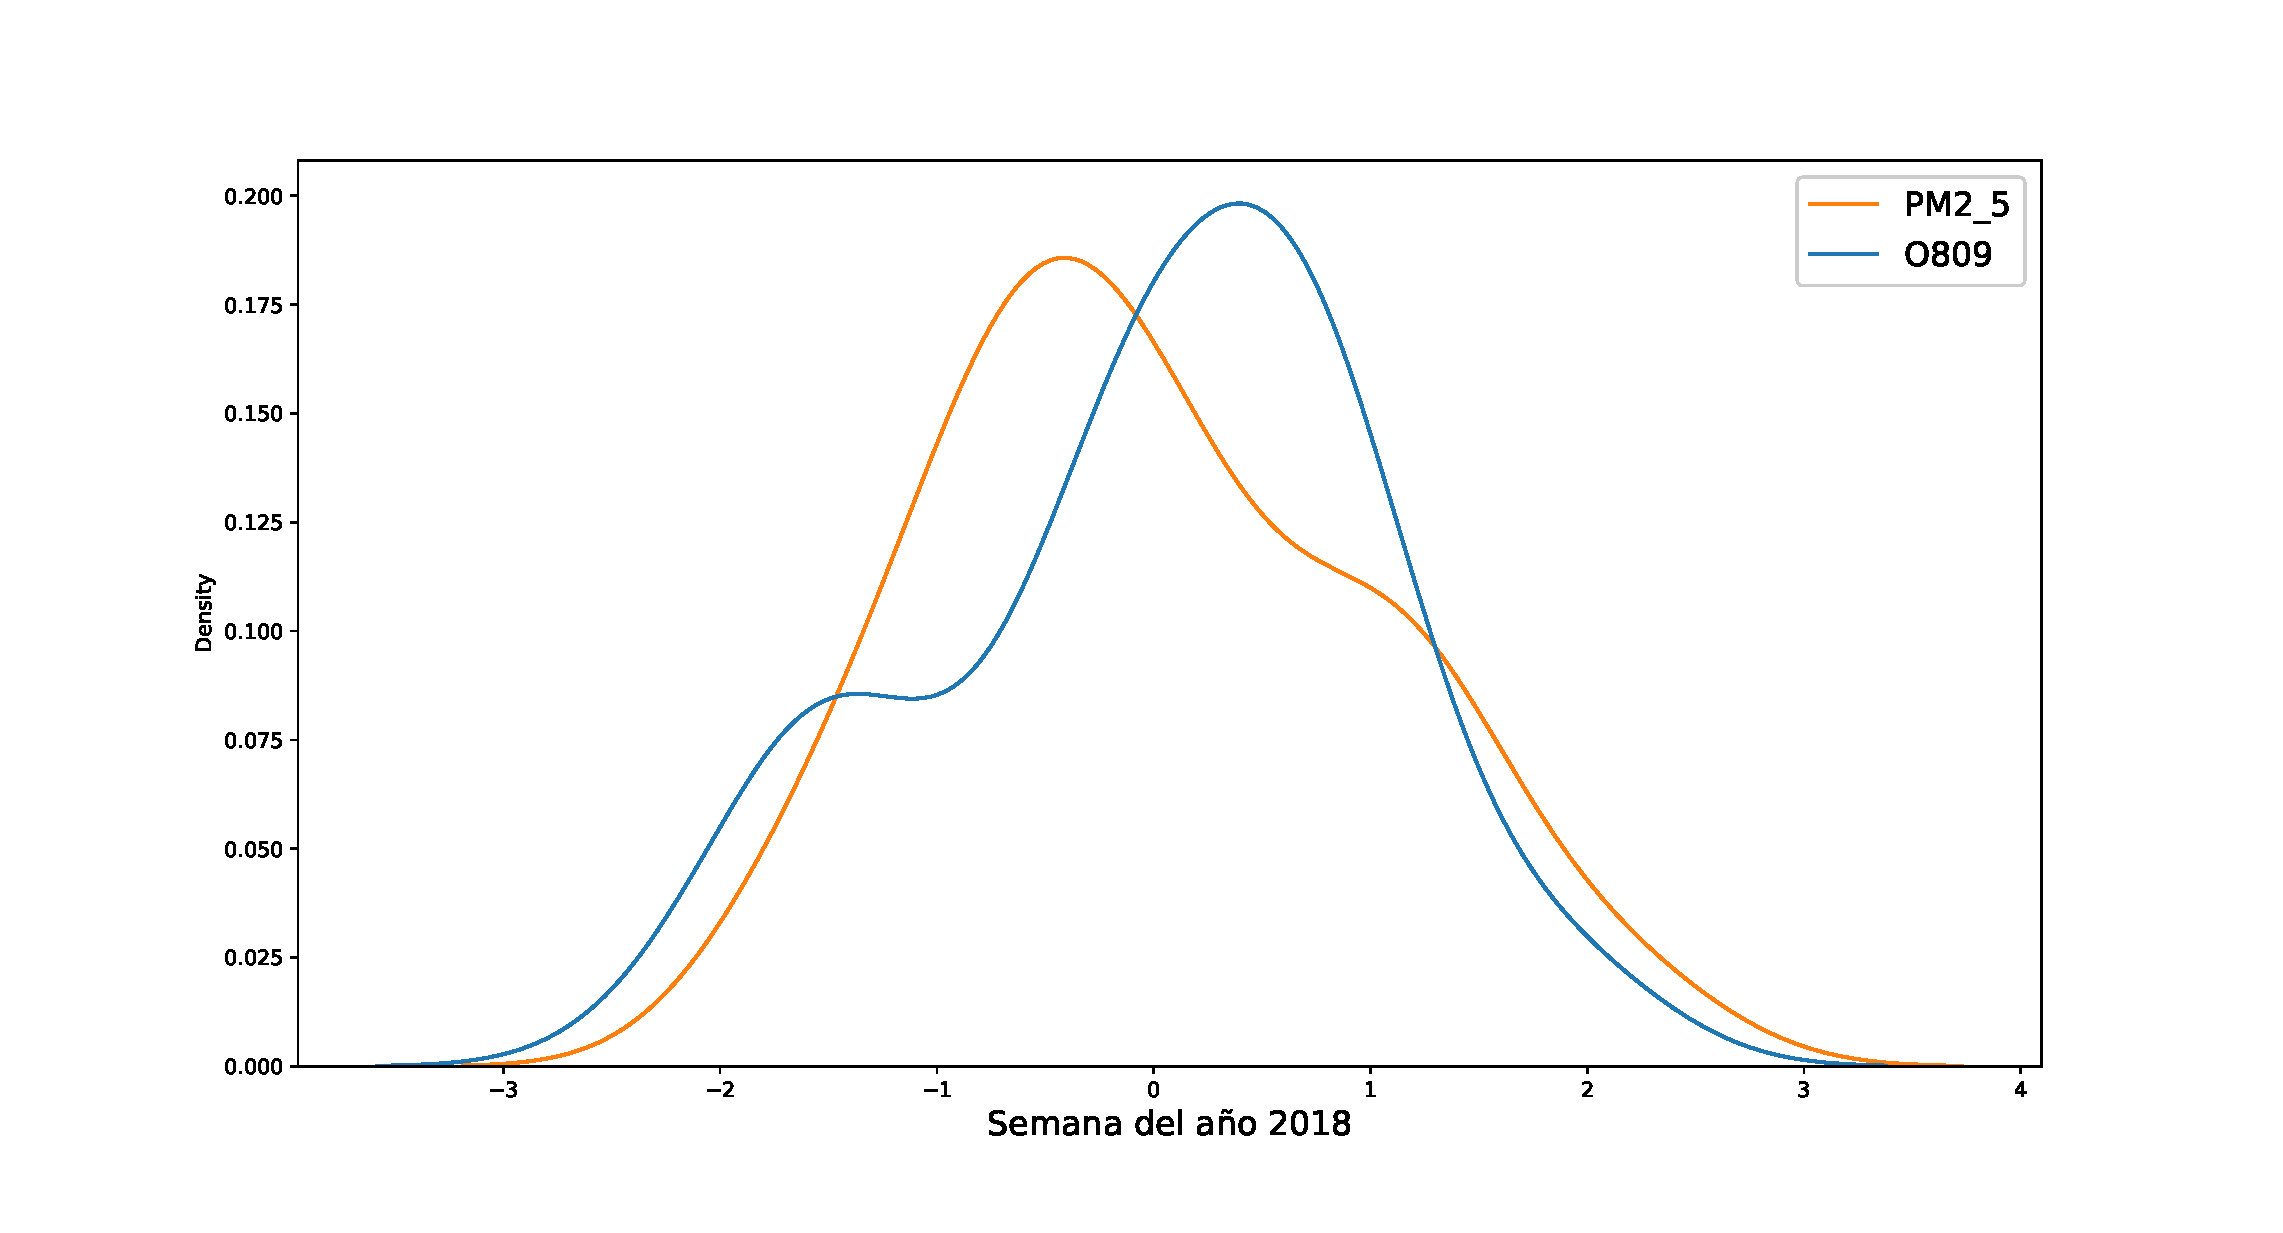
\includegraphics[trim=61 0 0 0,clip,width=1\textwidth]{PM2_5_O809_2018.eps}
   \end{center}
    \caption[Series de tiempo 2018 PM2.5 y O809]{Evolución de los niveles de PM2.5 y el número de egresos diagnosticados con la CIE O809 en el 2018.}
    \label{serie_de_tiempo_2018_PM25}
\end{figure}

\begin{table}[hbt!]
\centering
\caption{Resultados obtenidos PM2.5 2018}
\label{tab:Resultados obtenidos PM2.5 2018}
\vspace{0.5cm}
\begin{threeparttable}
\begin{tabular}{|c|c|c|c|c|}
	\hline
	CIE & $\rho$ & $R^2$ & Valor $p$ & $\epsilon$\\
	\hline
	O809 & -0.354 & 0.057 & 0.133 & 0.259 \\
	\hline
	O829 & 0.225 & 0.046 & 0.177 & 0.256 \\
	\hline
	K802 & 0.273 & 0.089 & 0.058 & 0.159 \\
	\hline
	O342 & -0.443 & 0.149 & 0.013 & 0.245 \\
	\hline
	N40X & -0.074 & 0.001 & 0.842 & 0.241 \\
	\hline
\end{tabular}
\begin{tablenotes}
\footnotesize
\item{$\rho$ = Coeficiente de correlación de Pearson}
\item{$\epsilon$ = RMSE para medir el error}
\end{tablenotes}
\end{threeparttable}
\end{table}

\begin{figure}[h!]
\setcounter{figure}{7} % por culpa de sciposter
\captionsetup{type=figure} % por culpa de sciposter
\begin{center}
   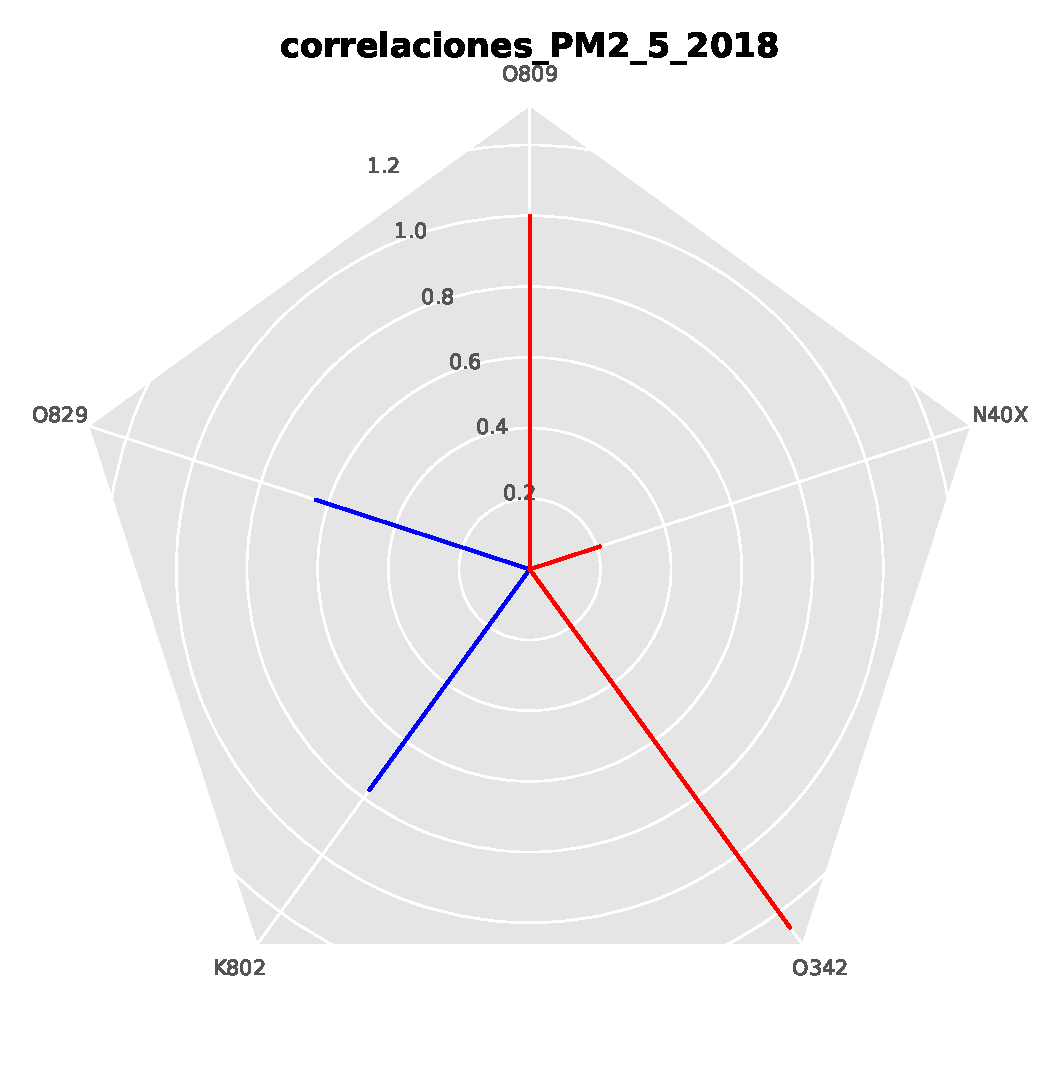
\includegraphics[trim=0 0 0 23,clip,width=1\textwidth]{spiderweb_correlaciones_PM2_5_2018}
   \end{center}
    \caption[Correlaciones 2018 PM2.5]{Correlaciones entre los niveles de PM2.5 y CIE en el 2018 donde el azul indica una correlación positiva y el rojo una correlación negativa.}
    \label{correlaciones_2018_PM25}
\end{figure}

\begin{table}[hbt!]
\caption{Resultados regresión lineal múltiple PM2.5 2018}
\label{tab:RRLM PM2.5 2018}
\begin{center}
\begin{tabular}{lclc}
\toprule
\textbf{Variable Dep.:}    &        $y$         & \textbf{  R$^2$:         } &     0.259   \\
\textbf{Modelo:}            &       OLS        & \textbf{Método:}           &  Mínimos cuadrados   \\
\textbf{Error:}            & 0.174  \\
\bottomrule
\end{tabular}
\begin{tabular}{lcccccc}
               & \textbf{coef} & \textbf{std err} & \textbf{$t$} & \textbf{P$> |$t$|$} & \textbf{[0.025} & \textbf{0.975]}  \\
\midrule
\textbf{const} &       0.7042  &        0.193     &     3.652  &         0.001        &        0.313    &        1.096     \\
\textbf{O809}  &      -0.0863  &        0.172     &    -0.501  &         0.620        &       -0.436    &        0.264     \\
\textbf{O829}  &      -0.1084  &        0.196     &    -0.553  &         0.584        &       -0.507    &        0.290     \\
\textbf{K802}  &       0.3006  &        0.153     &     1.964  &         0.058        &       -0.010    &        0.611     \\
\textbf{O342}  &      -0.3311  &        0.191     &    -1.733  &         0.092        &       -0.719    &        0.057     \\
\textbf{N40X}  &      -0.2053  &        0.154     &    -1.336  &         0.190        &       -0.517    &        0.107     \\
\bottomrule
\end{tabular}
\end{center}
\end{table}


\clearpage
\section{Discusión}
Como se puede observar, en todos los experimentos se obtiene una correlación entre -1 y 1 y diferente a 0, por lo tanto se pueden generar los modelos de regresión lineal.

En el Experimento A el error RMSE en los modelos de regresión lineal varía entre 0.152 y 0.294, lo cual indica que no todos los resultados alcanzan una fiabilidad mayor al 80\%, excepto en la CIE K802 en el año 2018 en la cual se encuentra el porcentaje de error más bajo. 
El valor de $R^2$ más alto en el año 2017 se encuentra en la CIE O759 con un valor $p$ de 0.029, sin embargo, en el modelo de regresión lineal múltiple se encuentra el valor de $R^2$ más alto para el contaminante PM10 en el año 2017. En el año 2018 el valor de $R^2$ más alto se encuentra en la CIE O342 con un valor $p$ de 0.044, sin embargo, en el modelo de regresión lineal múltiple se encuentra el valor de $R^2$ más alto para el contaminante PM10 en el año 2018.

En el Experimento B el error RMSE en los modelos de regresión lineal varía entre 0.159 y 0.278, lo cual indica que no todos los resultados alcanzan una fiabilidad mayor al 80\%, excepto en la CIE K802 en el año 2018 en la cual se encuentra el porcentaje de error más bajo.
El valor de $R^2$ más alto en el año 2017 se encuentra en la CIE O759 con un valor $p$ de 0.032, sin embargo, en el modelo de regresión lineal múltiple se encuentra el valor de $R^2$ más alto para el contaminante PM2.5 en el año 2017. En el año 2018 el valor de $R^2$ más alto se encuentra en la CIE O342 con un valor $p$ de 0.013, sin embargo, en el modelo de regresión lineal múltiple se encuentra el valor de $R^2$ más alto para el contaminante PM2.5 en el año 2018.

\clearpage
Todos los experimentos son ejecutados en \texttt{Jupyter Notebook} en una laptop con las especificaciones del cuadro \ref{tab:Especificaciones técnicas del PC}.

\begin{table}[H]
	{\centering
		\caption{Especificaciones técnicas del equipo de cómputo}
		\begin{tabular}{|c|c|c|}
			\hline
			Sistema Operativo & macOS Big Sur\\
			\hline
			Procesador & Apple M1\\
			\hline
			RAM & 8 GB RAM\\
			\hline
		\end{tabular}

	\label{tab:Especificaciones técnicas del PC}
	}
\end{table}

%\subsection{Experimento C: Niveles de NO$_x$}
%\subsubsection{Año 2015}
%\subsubsection{Año 2016}
%\subsubsection{Año 2017}
%\subsubsection{Año 2018}

%\subsection{Experimento D: Niveles de NO$_2$}
%\subsubsection{Año 2015}
%\subsubsection{Año 2016}
%\subsubsection{Año 2017}
%\subsubsection{Año 2018}